\begin{figure*}
  \vspace{-1.0em}
  \centering
  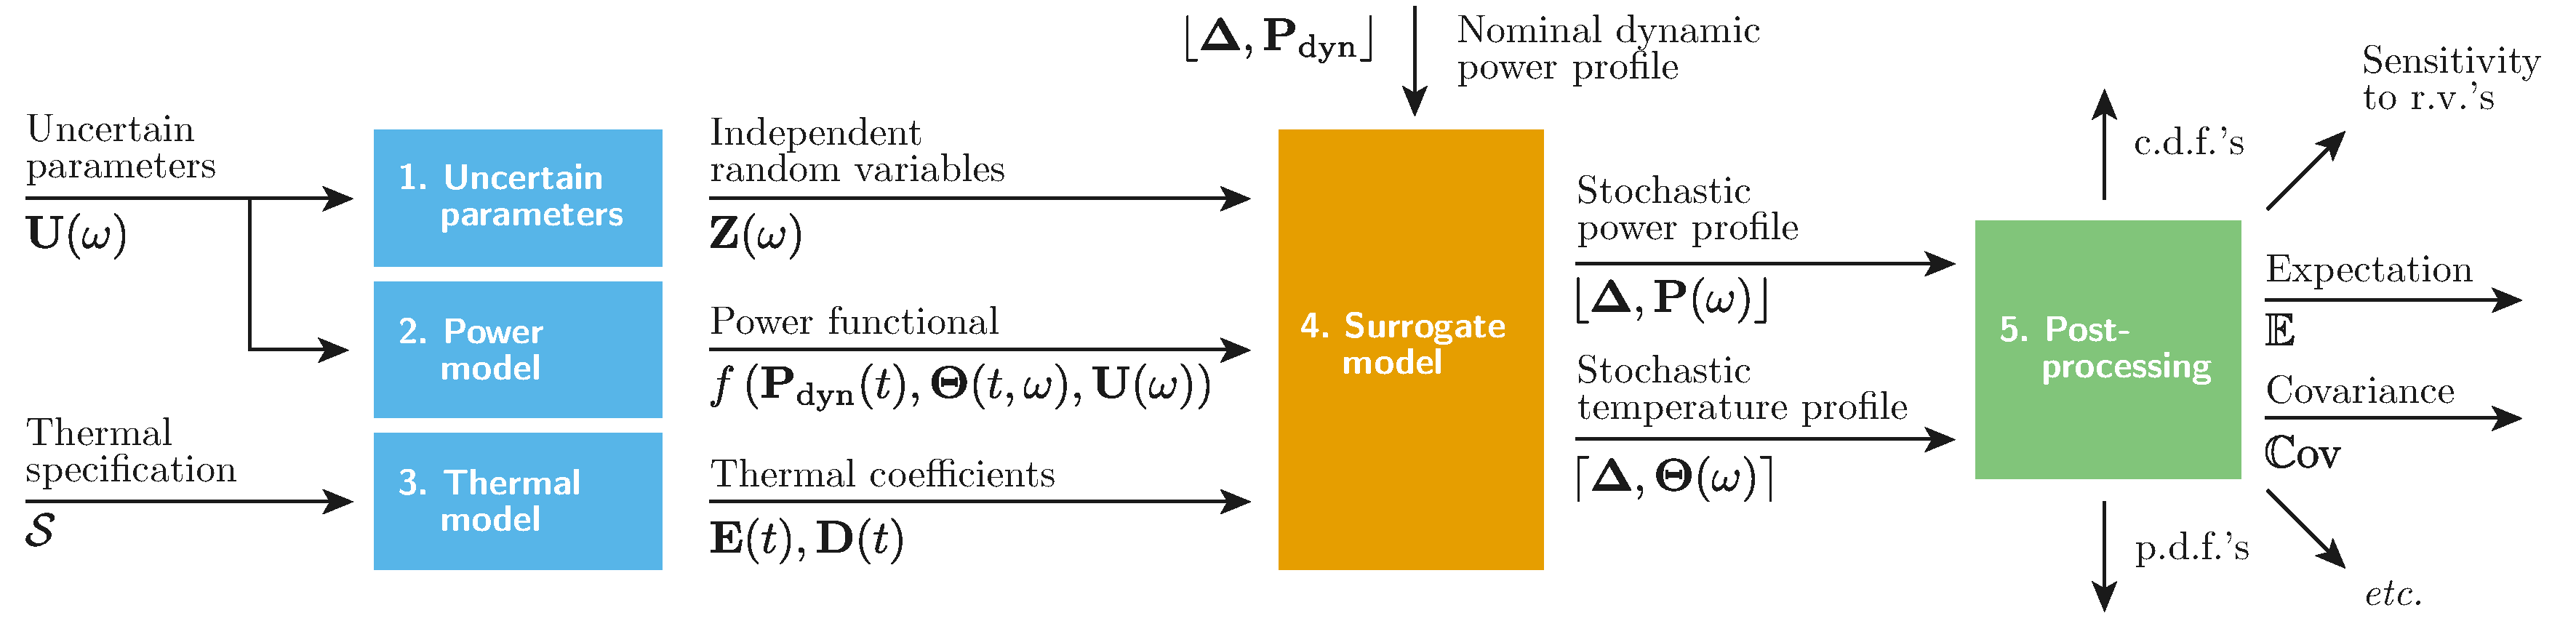
\includegraphics[width=1\textwidth]{include/assets/algorithm.pdf}
  \vspace{-1.0em}
  \caption{The structure of the proposed framework.}
  \flabel{algorithm}
  \vspace{-1.0em}
\end{figure*}

Consider a heterogeneous multiprocessor system that consists of $\cores$ processing elements and is equipped with a thermal package. The processing elements are the active components of the system identified at the intended level of granularity (processors, ALUs, caches, registers, \etc). The system is characterized by its power and temperature profiles, which we define as follows. A power profile $\profP$ over a time interval $\period$ is a tuple composed of a time partition $\part = \{ 0 = \t_0 < \dotsc < \t_{\steps} = \period \}$ with $\steps$ subintervals $\{ \dt_i = \t_i - \t_{i - 1} \}_{i = 1}^{\steps}$ and a matrix $\mP \in \real^{\cores \times \steps}$ that captures the power dissipation of all $\cores$ processing elements at the \emph{beginning} of all $\steps$ time intervals. The definition of a temperature profile $\profT$ is similar to the one for power except the fact that the temperature is tracked at the \emph{end} of the time intervals. This distinction is made merely for convenience and can be thought as: the power is applied first, and the temperature follows it with a time delay due to the inertia of the system.

Let $\system$ be a thermal specification of the system defined as a collection of temperature-related information: (a) the floorplans of the active layers of the chip; (b) the geometry of the thermal package; (c) the thermal parameters of the materials that the chip and package are made of; in this work, $\system$ is deterministic. In addition, the system depends on a set of uncertain parameters $\vU(\o)$---hereafter, $\o$ hints a random nature behind the quantity and will be formally defined later on---which manifest themselves in the deviation of the actual power dissipation from nominal values and, consequently, in the deviation of temperature from the one corresponding to the nominal power consumption. Therefore, we shall distinguish between deterministic and stochastic profiles. In the latter case, the power and temperature profiles are denoted by $\profP{\o}$ and $\profT{\o}$, respectively.

In this work, we aim to develop an UQ framework for power-temperature analysis (PTA) of multiprocessor systems where the power dissipation and temperature are unknown due to their dependency on the set of uncertain parameters $\vU(\o)$. The framework should be based on (a) a thermal specification of the platform $\system$; (b) a probability distribution of $\vU(\o)$, either joint or a set of marginals with a correlation matrix (discussed in \sref{uncertain-parameters}); (c) a model of the power dissipation as a function, possibly implicit, of $\vU(\o)$ (discussed in \sref{power-model}). Given a nominal dynamic power profile of the system $\profPdyn$, the framework should deliver the corresponding stochastic power $\profP{\o}$ and temperature $\profT{\o}$ profiles with the desired level of accuracy and a low computational cost. Here, we would like to point out that the last requirement is essential, and we emphasize it though out the article since the analysis of such a stochastic system is always possible to attain via the MC sampling protected by the central limit theorem. However, what makes a difference is the cost to pay as MC-based approaches are computationally expensive, often infeasible, in practice due to large numbers of simulations needed to obtain reliable estimates \cite{xiu2010, maitre2010, diaz-emparanza2002}.
